\documentclass{standalone}
\usepackage{tikz}
\usetikzlibrary{patterns, positioning}


\begin{document}
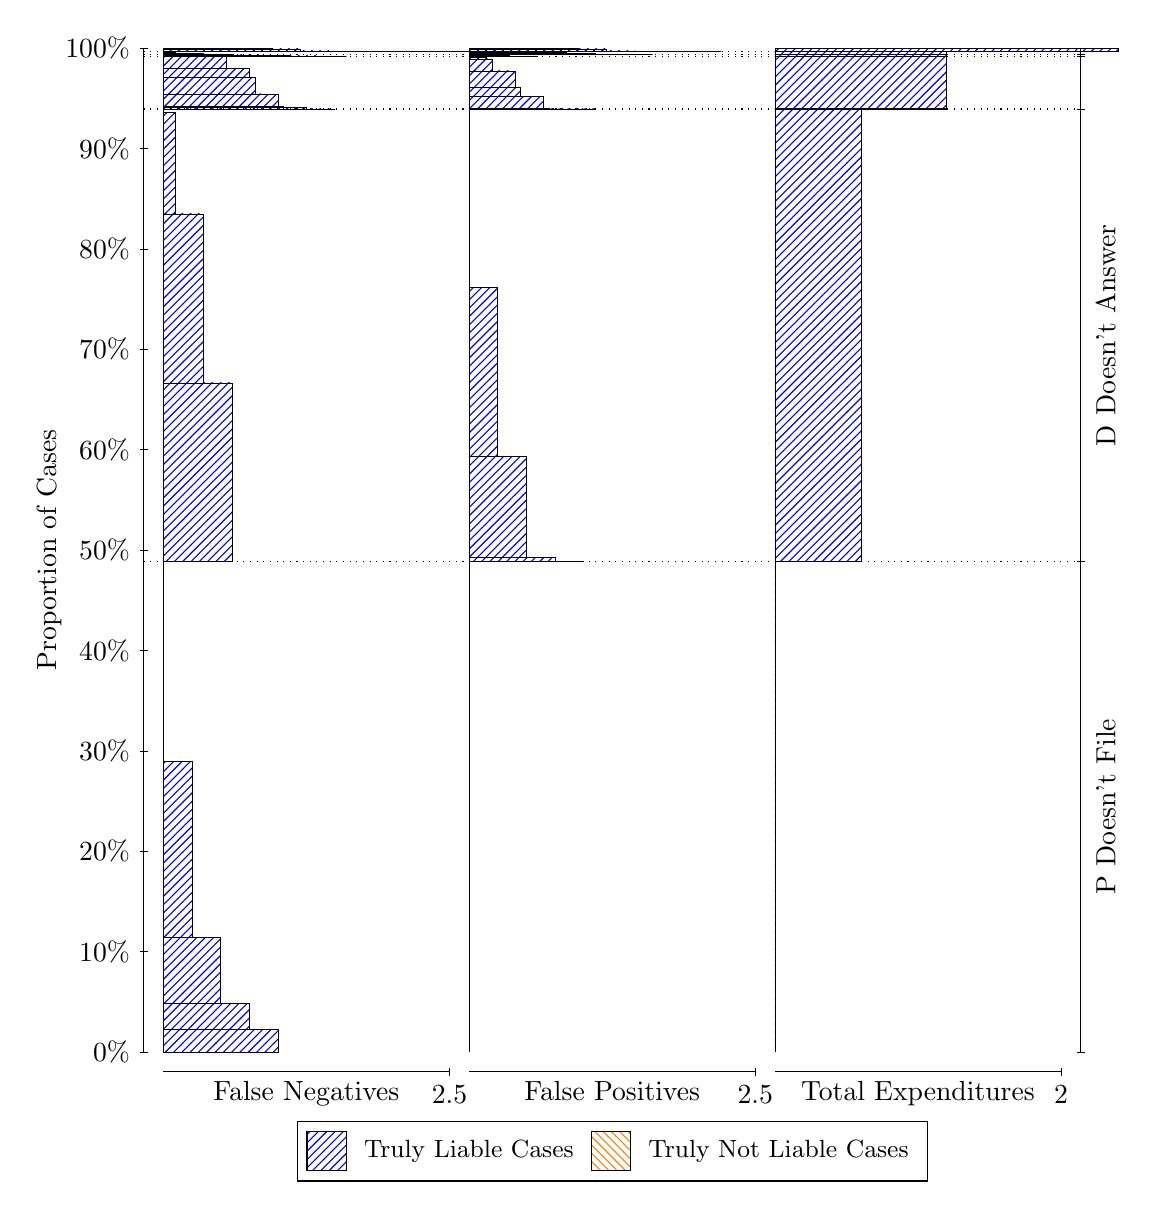
\begin{tikzpicture}
\draw[black, very thin] (1.5,1.75) -- (1.5,14.5);
\node[rotate=90, text=black, anchor=center] at (0.3, 8.125) {Proportion of Cases};
\draw[black, very thin] (1.45,1.75) -- (1.55,1.75);
\node[text=black, anchor=east] at (1.45, 1.75) {0\%};
\draw[black, very thin] (1.45,3.025) -- (1.55,3.025);
\node[text=black, anchor=east] at (1.45, 3.025) {10\%};
\draw[black, very thin] (1.45,4.3) -- (1.55,4.3);
\node[text=black, anchor=east] at (1.45, 4.3) {20\%};
\draw[black, very thin] (1.45,5.575) -- (1.55,5.575);
\node[text=black, anchor=east] at (1.45, 5.575) {30\%};
\draw[black, very thin] (1.45,6.85) -- (1.55,6.85);
\node[text=black, anchor=east] at (1.45, 6.85) {40\%};
\draw[black, very thin] (1.45,8.125) -- (1.55,8.125);
\node[text=black, anchor=east] at (1.45, 8.125) {50\%};
\draw[black, very thin] (1.45,9.4) -- (1.55,9.4);
\node[text=black, anchor=east] at (1.45, 9.4) {60\%};
\draw[black, very thin] (1.45,10.675) -- (1.55,10.675);
\node[text=black, anchor=east] at (1.45, 10.675) {70\%};
\draw[black, very thin] (1.45,11.95) -- (1.55,11.95);
\node[text=black, anchor=east] at (1.45, 11.95) {80\%};
\draw[black, very thin] (1.45,13.225) -- (1.55,13.225);
\node[text=black, anchor=east] at (1.45, 13.225) {90\%};
\draw[black, very thin] (1.45,14.5) -- (1.55,14.5);
\node[text=black, anchor=east] at (1.45, 14.5) {100\%};

\draw[black, very thin] (13.4,1.75) -- (13.4,14.5);
\draw[black, very thin] (13.35,1.75) -- (13.45,1.75);
\node[anchor=west] at (13.35, 1.75) {};
\draw[black, very thin] (13.35,7.9826) -- (13.45,7.9826);
\node[anchor=west] at (13.35, 7.9826) {};
\draw[black, very thin] (13.35,13.726) -- (13.45,13.726);
\node[anchor=west] at (13.35, 13.726) {};
\draw[black, very thin] (13.35,14.397) -- (13.45,14.397);
\node[anchor=west] at (13.35, 14.397) {};
\draw[black, very thin] (13.35,14.415) -- (13.45,14.415);
\node[anchor=west] at (13.35, 14.415) {};
\draw[black, very thin] (13.35,14.453) -- (13.45,14.453);
\node[anchor=west] at (13.35, 14.453) {};
\draw[black, very thin] (13.35,14.5) -- (13.45,14.5);
\node[anchor=west] at (13.35, 14.5) {};

\draw[black, very thin, pattern color=blue, pattern=north east lines] (1.75,1.75) rectangle (3.2033,2.0338);
\draw[black, very thin, pattern color=blue, pattern=north east lines] (1.75,2.0338) rectangle (2.84,2.3648);
\draw[black, very thin, pattern color=blue, pattern=north east lines] (1.75,2.3648) rectangle (2.4767,3.2012);
\draw[black, very thin, pattern color=blue, pattern=north east lines] (1.75,3.2012) rectangle (2.1133,5.4358);
\draw[black, very thin, pattern color=orange, pattern=north west lines] (1.75,5.4358) rectangle (1.75,5.4358);
\draw[black, very thin, pattern color=blue, pattern=north east lines] (1.75,5.4358) rectangle (1.75,7.9826);
\draw[black, very thin, pattern color=blue, pattern=north east lines] (1.75,7.9826) rectangle (2.622,10.248);
\draw[black, very thin, pattern color=blue, pattern=north east lines] (1.75,10.248) rectangle (2.2587,12.393);
\draw[black, very thin, pattern color=blue, pattern=north east lines] (1.75,12.393) rectangle (1.8953,13.681);
\draw[black, very thin, pattern color=orange, pattern=north west lines] (1.75,13.681) rectangle (1.75,13.681);
\draw[black, very thin, pattern color=blue, pattern=north east lines] (1.75,13.681) rectangle (1.75,13.726);
\draw[black, very thin, pattern color=blue, pattern=north east lines] (1.75,13.726) rectangle (3.93,13.726);
\draw[black, very thin, pattern color=blue, pattern=north east lines] (1.75,13.726) rectangle (3.6393,13.726);
\draw[black, very thin, pattern color=blue, pattern=north east lines] (1.75,13.726) rectangle (3.5667,13.742);
\draw[black, very thin, pattern color=blue, pattern=north east lines] (1.75,13.742) rectangle (3.3487,13.742);
\draw[black, very thin, pattern color=blue, pattern=north east lines] (1.75,13.742) rectangle (3.276,13.761);
\draw[black, very thin, pattern color=blue, pattern=north east lines] (1.75,13.761) rectangle (3.2033,13.913);
\draw[black, very thin, pattern color=blue, pattern=north east lines] (1.75,13.913) rectangle (2.9853,13.918);
\draw[black, very thin, pattern color=blue, pattern=north east lines] (1.75,13.918) rectangle (2.9127,14.127);
\draw[black, very thin, pattern color=blue, pattern=north east lines] (1.75,14.127) rectangle (2.84,14.237);
\draw[black, very thin, pattern color=blue, pattern=north east lines] (1.75,14.237) rectangle (2.622,14.24);
\draw[black, very thin, pattern color=blue, pattern=north east lines] (1.75,14.24) rectangle (2.5493,14.394);
\draw[black, very thin, pattern color=blue, pattern=north east lines] (1.75,14.394) rectangle (2.4767,14.395);
\draw[black, very thin, pattern color=blue, pattern=north east lines] (1.75,14.395) rectangle (2.2587,14.395);
\draw[black, very thin, pattern color=blue, pattern=north east lines] (1.75,14.395) rectangle (2.186,14.397);
\draw[black, very thin, pattern color=blue, pattern=north east lines] (1.75,14.397) rectangle (1.8953,14.397);
\draw[black, very thin, pattern color=orange, pattern=north west lines] (1.75,14.397) rectangle (1.75,14.397);
\draw[black, very thin, pattern color=blue, pattern=north east lines] (1.75,14.397) rectangle (4.0753,14.397);
\draw[black, very thin, pattern color=blue, pattern=north east lines] (1.75,14.397) rectangle (3.712,14.4);
\draw[black, very thin, pattern color=blue, pattern=north east lines] (1.75,14.4) rectangle (3.3487,14.409);
\draw[black, very thin, pattern color=blue, pattern=north east lines] (1.75,14.409) rectangle (2.9853,14.414);
\draw[black, very thin, pattern color=blue, pattern=north east lines] (1.75,14.414) rectangle (2.622,14.415);
\draw[black, very thin, pattern color=orange, pattern=north west lines] (1.75,14.415) rectangle (1.75,14.415);
\draw[black, very thin, pattern color=blue, pattern=north east lines] (1.75,14.415) rectangle (2.622,14.415);
\draw[black, very thin, pattern color=blue, pattern=north east lines] (1.75,14.415) rectangle (2.2587,14.436);
\draw[black, very thin, pattern color=blue, pattern=north east lines] (1.75,14.436) rectangle (1.8953,14.452);
\draw[black, very thin, pattern color=orange, pattern=north west lines] (1.75,14.452) rectangle (1.75,14.452);
\draw[black, very thin, pattern color=blue, pattern=north east lines] (1.75,14.452) rectangle (1.75,14.453);
\draw[black, very thin, pattern color=blue, pattern=north east lines] (1.75,14.453) rectangle (5.8193,14.453);
\draw[black, very thin, pattern color=blue, pattern=north east lines] (1.75,14.453) rectangle (5.456,14.453);
\draw[black, very thin, pattern color=blue, pattern=north east lines] (1.75,14.453) rectangle (5.0927,14.453);
\draw[black, very thin, pattern color=blue, pattern=north east lines] (1.75,14.453) rectangle (4.7293,14.456);
\draw[black, very thin, pattern color=blue, pattern=north east lines] (1.75,14.456) rectangle (4.584,14.456);
\draw[black, very thin, pattern color=blue, pattern=north east lines] (1.75,14.456) rectangle (4.366,14.456);
\draw[black, very thin, pattern color=blue, pattern=north east lines] (1.75,14.456) rectangle (4.2207,14.457);
\draw[black, very thin, pattern color=blue, pattern=north east lines] (1.75,14.457) rectangle (4.0027,14.457);
\draw[black, very thin, pattern color=blue, pattern=north east lines] (1.75,14.457) rectangle (3.8573,14.465);
\draw[black, very thin, pattern color=blue, pattern=north east lines] (1.75,14.465) rectangle (3.494,14.488);
\draw[black, very thin, pattern color=blue, pattern=north east lines] (1.75,14.488) rectangle (3.1307,14.499);
\draw[black, very thin, pattern color=blue, pattern=north east lines] (1.75,14.499) rectangle (2.7673,14.5);
\draw[black, very thin, pattern color=blue, pattern=north east lines] (1.75,14.5) rectangle (2.404,14.5);
\draw[black, very thin, pattern color=blue, pattern=north east lines] (1.75,14.5) rectangle (2.0407,14.5);
\draw[black, very thin, pattern color=orange, pattern=north west lines] (1.75,14.5) rectangle (1.75,14.5);
\draw[black, very thin, pattern color=orange, pattern=north west lines] (5.6333,1.75) rectangle (5.6333,1.75);
\draw[black, very thin, pattern color=blue, pattern=north east lines] (5.6333,1.75) rectangle (5.6333,7.9826);
\draw[black, very thin, pattern color=orange, pattern=north west lines] (5.6333,7.9826) rectangle (7.0867,7.9826);
\draw[black, very thin, pattern color=blue, pattern=north east lines] (5.6333,7.9826) rectangle (7.0867,7.9826);
\draw[black, very thin, pattern color=blue, pattern=north east lines] (5.6333,7.9826) rectangle (6.7233,8.0273);
\draw[black, very thin, pattern color=blue, pattern=north east lines] (5.6333,8.0273) rectangle (6.36,9.3156);
\draw[black, very thin, pattern color=blue, pattern=north east lines] (5.6333,9.3156) rectangle (5.9967,11.46);
\draw[black, very thin, pattern color=blue, pattern=north east lines] (5.6333,11.46) rectangle (5.6333,13.726);
\draw[black, very thin, pattern color=orange, pattern=north west lines] (5.6333,13.726) rectangle (7.232,13.726);
\draw[black, very thin, pattern color=blue, pattern=north east lines] (5.6333,13.726) rectangle (7.232,13.726);
\draw[black, very thin, pattern color=orange, pattern=north west lines] (5.6333,13.726) rectangle (6.9413,13.726);
\draw[black, very thin, pattern color=blue, pattern=north east lines] (5.6333,13.726) rectangle (6.9413,13.728);
\draw[black, very thin, pattern color=blue, pattern=north east lines] (5.6333,13.728) rectangle (6.8687,13.728);
\draw[black, very thin, pattern color=orange, pattern=north west lines] (5.6333,13.728) rectangle (6.6507,13.728);
\draw[black, very thin, pattern color=blue, pattern=north east lines] (5.6333,13.728) rectangle (6.6507,13.729);
\draw[black, very thin, pattern color=blue, pattern=north east lines] (5.6333,13.729) rectangle (6.578,13.883);
\draw[black, very thin, pattern color=blue, pattern=north east lines] (5.6333,13.883) rectangle (6.5053,13.886);
\draw[black, very thin, pattern color=blue, pattern=north east lines] (5.6333,13.886) rectangle (6.2873,13.996);
\draw[black, very thin, pattern color=blue, pattern=north east lines] (5.6333,13.996) rectangle (6.2147,14.205);
\draw[black, very thin, pattern color=blue, pattern=north east lines] (5.6333,14.205) rectangle (6.142,14.21);
\draw[black, very thin, pattern color=blue, pattern=north east lines] (5.6333,14.21) rectangle (5.924,14.362);
\draw[black, very thin, pattern color=blue, pattern=north east lines] (5.6333,14.362) rectangle (5.8513,14.38);
\draw[black, very thin, pattern color=blue, pattern=north east lines] (5.6333,14.38) rectangle (5.7787,14.381);
\draw[black, very thin, pattern color=blue, pattern=north east lines] (5.6333,14.381) rectangle (5.6333,14.397);
\draw[black, very thin, pattern color=orange, pattern=north west lines] (5.6333,14.397) rectangle (6.5053,14.397);
\draw[black, very thin, pattern color=blue, pattern=north east lines] (5.6333,14.397) rectangle (6.5053,14.397);
\draw[black, very thin, pattern color=blue, pattern=north east lines] (5.6333,14.397) rectangle (6.142,14.402);
\draw[black, very thin, pattern color=blue, pattern=north east lines] (5.6333,14.402) rectangle (5.7787,14.411);
\draw[black, very thin, pattern color=blue, pattern=north east lines] (5.6333,14.411) rectangle (5.6333,14.415);
\draw[black, very thin, pattern color=orange, pattern=north west lines] (5.6333,14.415) rectangle (7.9587,14.415);
\draw[black, very thin, pattern color=blue, pattern=north east lines] (5.6333,14.415) rectangle (7.9587,14.415);
\draw[black, very thin, pattern color=blue, pattern=north east lines] (5.6333,14.415) rectangle (7.5953,14.415);
\draw[black, very thin, pattern color=blue, pattern=north east lines] (5.6333,14.415) rectangle (7.232,14.431);
\draw[black, very thin, pattern color=blue, pattern=north east lines] (5.6333,14.431) rectangle (6.8687,14.452);
\draw[black, very thin, pattern color=blue, pattern=north east lines] (5.6333,14.452) rectangle (6.5053,14.453);
\draw[black, very thin, pattern color=orange, pattern=north west lines] (5.6333,14.453) rectangle (8.8307,14.453);
\draw[black, very thin, pattern color=blue, pattern=north east lines] (5.6333,14.453) rectangle (8.8307,14.453);
\draw[black, very thin, pattern color=blue, pattern=north east lines] (5.6333,14.453) rectangle (8.4673,14.453);
\draw[black, very thin, pattern color=orange, pattern=north west lines] (5.6333,14.453) rectangle (8.4673,14.453);
\draw[black, very thin, pattern color=blue, pattern=north east lines] (5.6333,14.453) rectangle (8.4673,14.453);
\draw[black, very thin, pattern color=blue, pattern=north east lines] (5.6333,14.453) rectangle (8.104,14.453);
\draw[black, very thin, pattern color=orange, pattern=north west lines] (5.6333,14.453) rectangle (8.104,14.453);
\draw[black, very thin, pattern color=blue, pattern=north east lines] (5.6333,14.453) rectangle (8.104,14.453);
\draw[black, very thin, pattern color=blue, pattern=north east lines] (5.6333,14.453) rectangle (7.7407,14.456);
\draw[black, very thin, pattern color=orange, pattern=north west lines] (5.6333,14.456) rectangle (7.7407,14.456);
\draw[black, very thin, pattern color=blue, pattern=north east lines] (5.6333,14.456) rectangle (7.7407,14.464);
\draw[black, very thin, pattern color=blue, pattern=north east lines] (5.6333,14.464) rectangle (7.3773,14.464);
\draw[black, very thin, pattern color=blue, pattern=north east lines] (5.6333,14.464) rectangle (7.3773,14.488);
\draw[black, very thin, pattern color=blue, pattern=north east lines] (5.6333,14.488) rectangle (7.014,14.496);
\draw[black, very thin, pattern color=orange, pattern=north west lines] (5.6333,14.496) rectangle (6.8687,14.496);
\draw[black, very thin, pattern color=blue, pattern=north east lines] (5.6333,14.496) rectangle (6.8687,14.496);
\draw[black, very thin, pattern color=blue, pattern=north east lines] (5.6333,14.496) rectangle (6.6507,14.496);
\draw[black, very thin, pattern color=orange, pattern=north west lines] (5.6333,14.496) rectangle (6.5053,14.496);
\draw[black, very thin, pattern color=blue, pattern=north east lines] (5.6333,14.496) rectangle (6.5053,14.496);
\draw[black, very thin, pattern color=blue, pattern=north east lines] (5.6333,14.496) rectangle (6.2873,14.496);
\draw[black, very thin, pattern color=blue, pattern=north east lines] (5.6333,14.496) rectangle (6.142,14.499);
\draw[black, very thin, pattern color=blue, pattern=north east lines] (5.6333,14.499) rectangle (5.7787,14.5);
\draw[black, very thin, pattern color=blue, pattern=north east lines] (5.6333,14.5) rectangle (5.6333,14.5);
\draw[black, very thin, pattern color=orange, pattern=north west lines] (9.5167,1.75) rectangle (9.5167,1.75);
\draw[black, very thin, pattern color=blue, pattern=north east lines] (9.5167,1.75) rectangle (9.5167,7.9826);
\draw[black, very thin, pattern color=orange, pattern=north west lines] (9.5167,7.9826) rectangle (10.607,7.9826);
\draw[black, very thin, pattern color=blue, pattern=north east lines] (9.5167,7.9826) rectangle (10.607,13.726);
\draw[black, very thin, pattern color=orange, pattern=north west lines] (9.5167,13.726) rectangle (11.697,13.726);
\draw[black, very thin, pattern color=blue, pattern=north east lines] (9.5167,13.726) rectangle (11.697,13.735);
\draw[black, very thin, pattern color=orange, pattern=north west lines] (9.5167,13.735) rectangle (11.697,13.735);
\draw[black, very thin, pattern color=blue, pattern=north east lines] (9.5167,13.735) rectangle (11.697,14.397);
\draw[black, very thin, pattern color=orange, pattern=north west lines] (9.5167,14.397) rectangle (11.697,14.397);
\draw[black, very thin, pattern color=blue, pattern=north east lines] (9.5167,14.397) rectangle (11.697,14.415);
\draw[black, very thin, pattern color=orange, pattern=north west lines] (9.5167,14.415) rectangle (11.697,14.415);
\draw[black, very thin, pattern color=blue, pattern=north east lines] (9.5167,14.415) rectangle (11.697,14.453);
\draw[black, very thin, pattern color=orange, pattern=north west lines] (9.5167,14.453) rectangle (13.877,14.453);
\draw[black, very thin, pattern color=blue, pattern=north east lines] (9.5167,14.453) rectangle (13.877,14.456);
\draw[black, very thin, pattern color=orange, pattern=north west lines] (9.5167,14.456) rectangle (13.877,14.456);
\draw[black, very thin, pattern color=blue, pattern=north east lines] (9.5167,14.456) rectangle (13.877,14.5);
\draw[black, dotted] (1.5,7.9826) -- (13.4,7.9826);
\draw[black, dotted] (1.5,13.726) -- (13.4,13.726);
\draw[black, dotted] (1.5,14.397) -- (13.4,14.397);
\draw[black, dotted] (1.5,14.415) -- (13.4,14.415);
\draw[black, dotted] (1.5,14.453) -- (13.4,14.453);
\draw[black, very thin] (1.75,1.5) -- (5.3833,1.5);
\node[text=black, anchor=north] at (3.5667, 1.5) {False Negatives};
\draw[black, very thin] (5.3833,1.45) -- (5.3833,1.55);
\node[text=black, anchor=north] at (5.3833, 1.45) {2.5};

\draw[black, very thin] (5.6333,1.5) -- (9.2667,1.5);
\node[text=black, anchor=north] at (7.45, 1.5) {False Positives};
\draw[black, very thin] (9.2667,1.45) -- (9.2667,1.55);
\node[text=black, anchor=north] at (9.2667, 1.45) {2.5};

\draw[black, very thin] (9.5167,1.5) -- (13.15,1.5);
\node[text=black, anchor=north] at (11.333, 1.5) {Total Expenditures};
\draw[black, very thin] (13.15,1.45) -- (13.15,1.55);
\node[text=black, anchor=north] at (13.15, 1.45) {2};

\node[text=black, centered, rotate=90] at (13.72, 4.8663) {P Doesn't File};
\node[text=black, centered, rotate=90] at (13.72, 10.854) {D Doesn't Answer};





\draw (7.449999999999999,1.5) node[draw=none] (baseCoordinate) {};
\begin{scope}[align=center]
        \matrix[scale=0.5, draw=black, below=0.5cm of baseCoordinate, nodes={draw}, column sep=0.1cm]{
            \node[rectangle, draw, minimum width=0.5cm, minimum height=0.5cm, pattern color=blue, pattern=north east lines] {}; &
            \node[draw=none, font=\small, text=black] (B) {Truly Liable Cases}; &
            \node[rectangle, draw, minimum width=0.5cm, minimum height=0.5cm, pattern color=orange, pattern=north west lines] {}; &
            \node[draw=none, font=\small, text=black] (B) {Truly Not Liable Cases}; \\
            };
\end{scope}

\end{tikzpicture}
\end{document}